\chapter{Design}
This chapter presents the design of the project. The overview of the design is presented in the figure \ref{fig:design}. The project is divided into several components, which are described further in this chapter. The assignment poses several constraints on the used technology, which ultimately influences the overall design. Furthermore, there is a number of design criteria to consider:
\begin{itemize}[noitemsep]
    \item nature of the input data
    \item clarity and usability of the system
    \item nature of the supported presentation formats
    \item computational and memory efficiency
    \item expandability of the system
\end{itemize}

\begin{figure}[h]
    \centering
    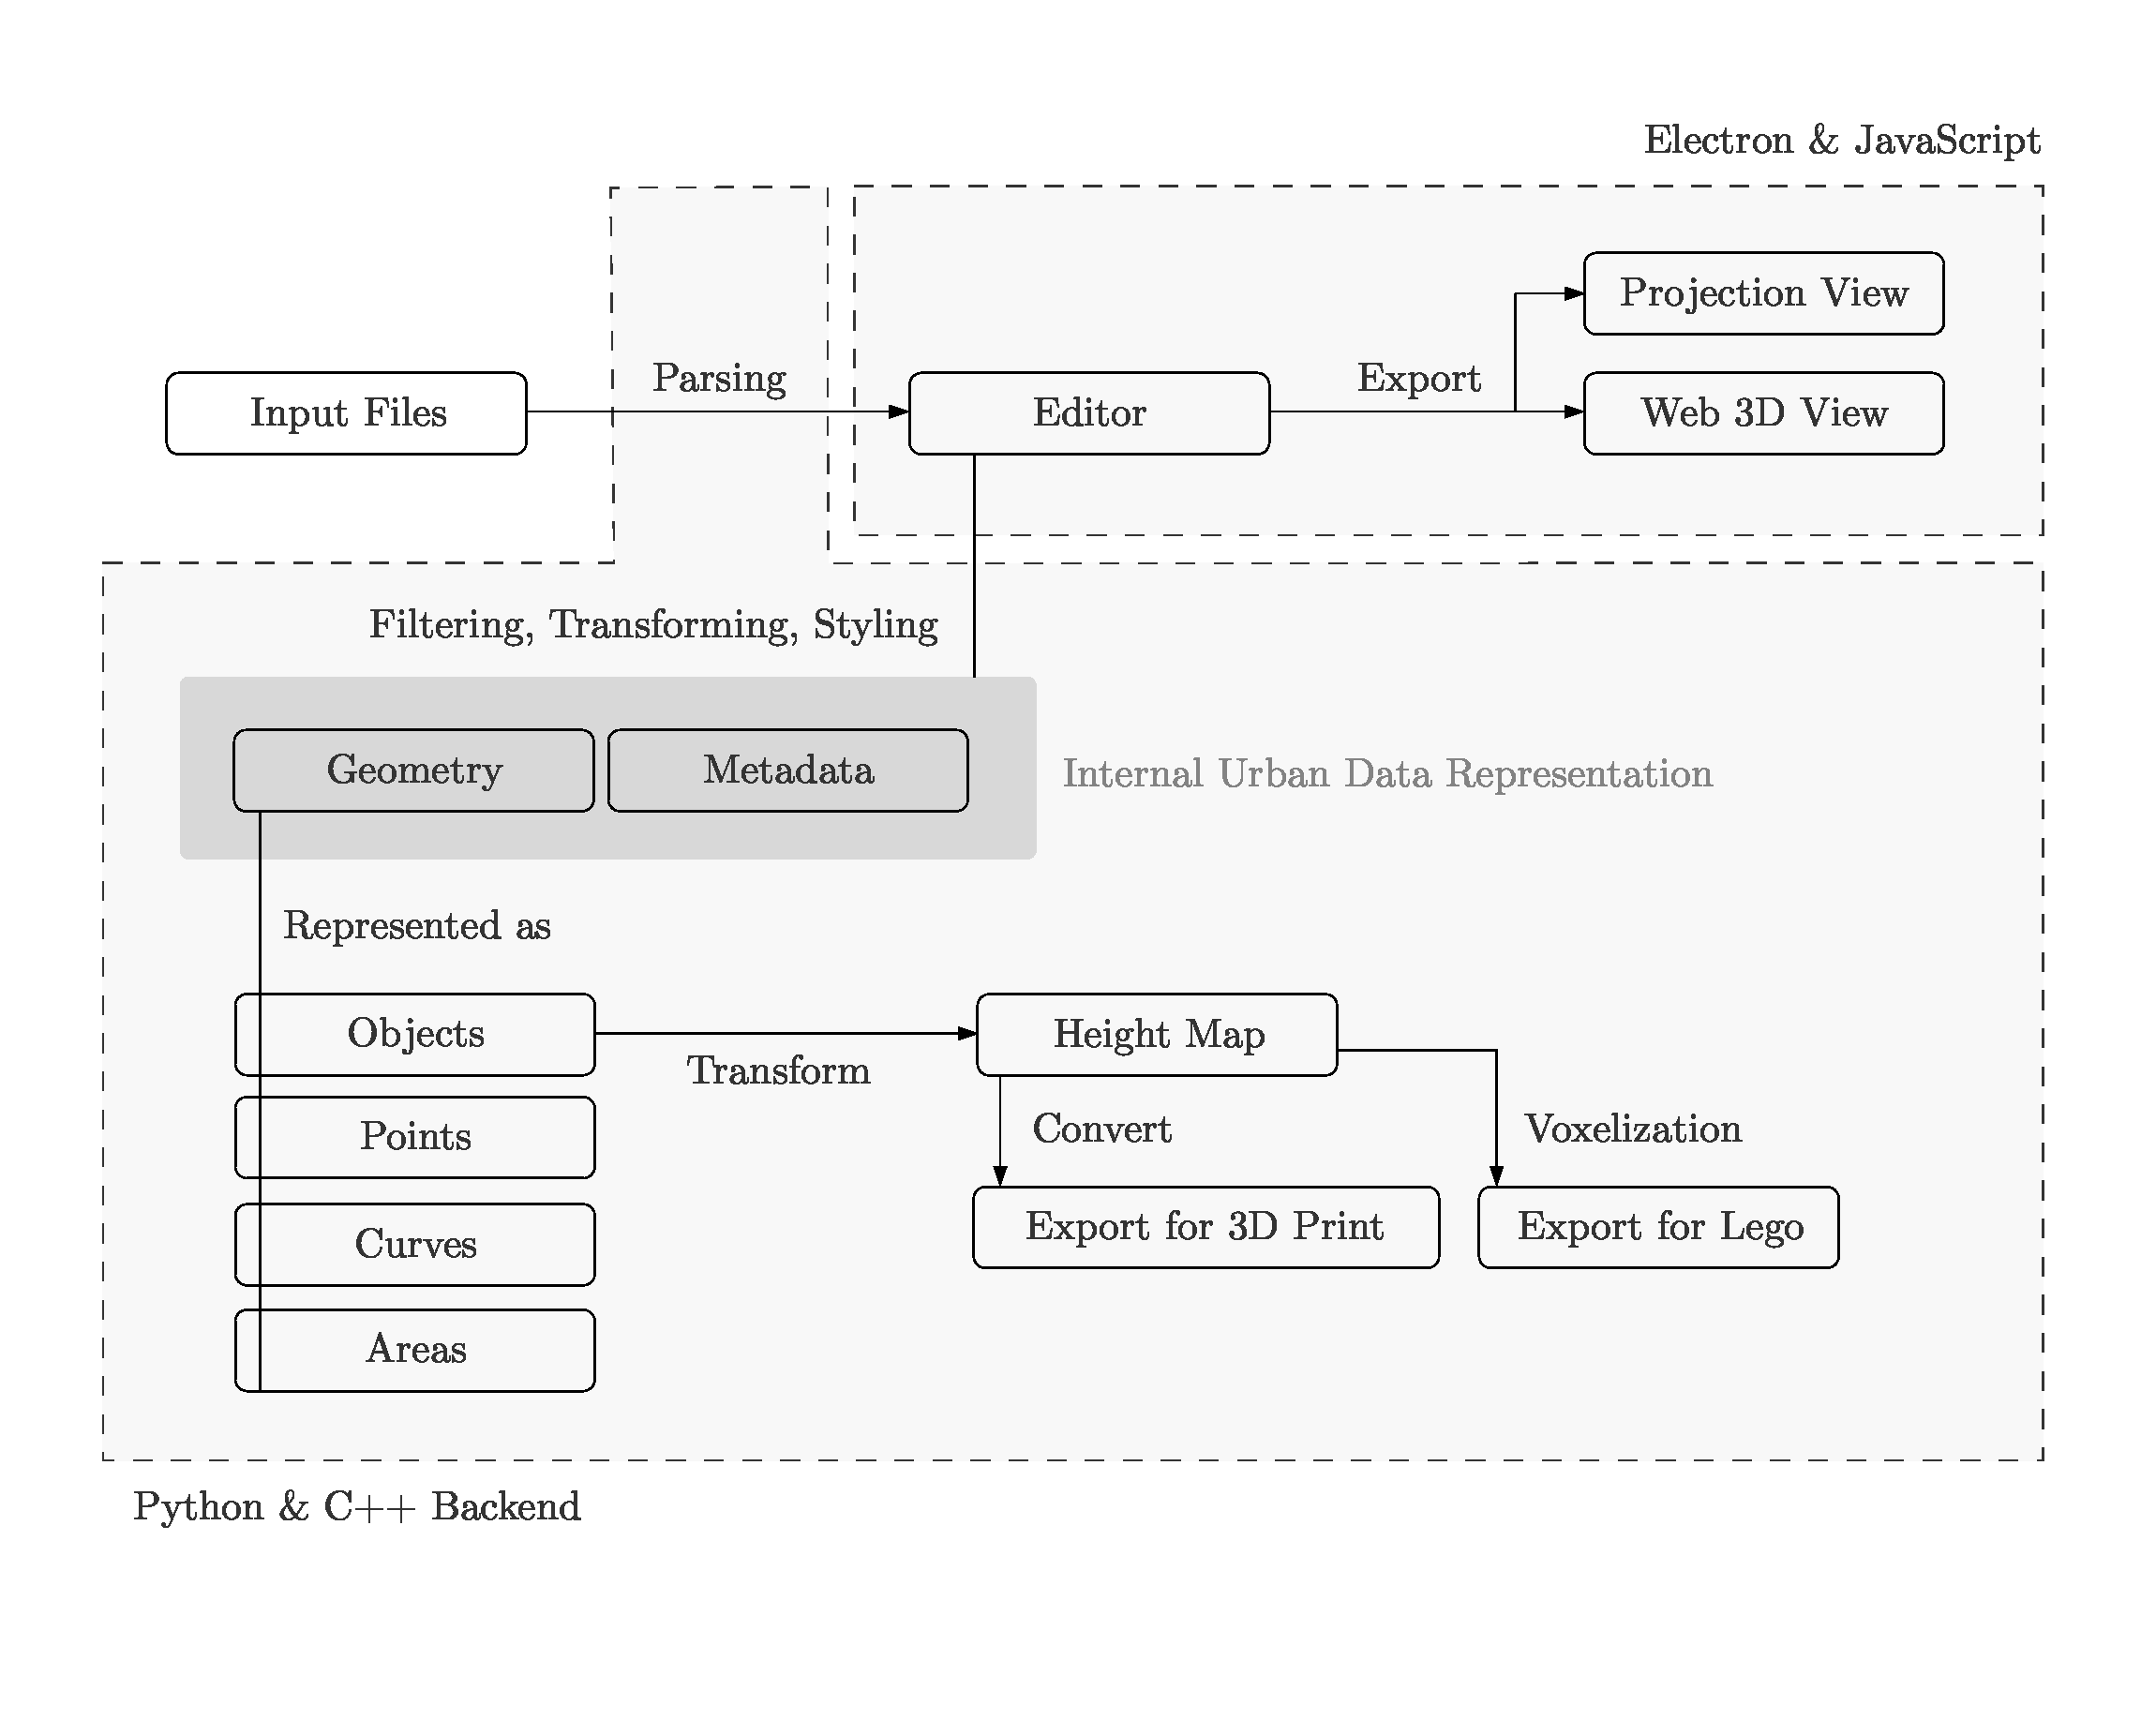
\includegraphics[width=\linewidth]{figures/app.pdf}
    \caption{Illustration of the proposed design}
    \label{fig:design}
\end{figure}

\section{Design Outline}
Based on the requirements and goals presented in the section \ref{sec:goals}, it is possible to divide the proposed  visualization system into three independent components:
\begin{description}[noitemsep]
    \item[Editor] The editor component handles the user interface and provides an easy way to assemble a custom visualization pipeline; the controls are based on visual programming principles.
    \item[Data Processing] The data processing component is an independent part of the system; it filters and transforms the urban data based on the pipeline description provided by the editor, the essential feature of the component is its modularity.
    \item[Web and Projection Views] The web and projection view components act as the data viewport, where the actual interactive visualization is presented to the user.  
\end{description}

The key principle of the design is \textit{modularity}. Since it is not possible to define a complete set of functionalities sufficient for every project, the system is designed to allow seamless integration of new functional elements, especially in the data processing component. Since the components are mostly independent, it is possible to implement each of them using different technology. The choice of the technology is based on the design criteria presented at the beginning of this chapter, as well as on the initial requirements. The design of the visualization pipeline consists of the following steps:
\begin{enumerate}
    \item selected files are imported into the editor; the files are preprocessed into the internal data representation in the background,
    \item user assembles the filtering and mapping parts of the visualization pipeline in the editor,
    \item the editor generates a graph of processing steps,
    \item the data processing component parses the graph and processes the input data,
    \item and output files are generated, including exports for views and model production.  
\end{enumerate}

\section{Input Formats and Data Representation}
\label{sec:inputrepres}
A list of urban data formats is presented in the section \ref{sec:formats}. From the developer perspective, the most accessible formats are CityGML, CityJSON, and GeoJSON. Since both CityGML and CityJSON are quite extensive formats, it is not desirable to reimplement the file readers. 

As the widely used readers of CityGML and CityJSON are written in different programming languages, it is necessary to choose the supported formats with respect to the implementation of the processing component. Luckily, the structure of the CityJSON and CityGML is almost identical; the only difference is in the base format (JSON vs. XML). Therefore, the data processing component can be implemented in Python or Java. 

The design of the internal data representation uses a simple model of geometry accompanied by metadata. Both CityGML and CityJSON formats use a range of spatial elements to represent the geographical entities. From the perspective of the urban data visualization, it is possible to limit the geometrical representation to the following elements:
\begin{description}[noitemsep]
    \item[Points] Points can represent a spatial feature, such as small points of interest, geotagged content, etc.
    \item[Curves] Curves, internally represented as line segments, can represent streets, roads, waterways, technical networks, etc.
    \item[Areas] Areas represent strictly 2D features, such as zones (parks, squares, parking lots, brownfields, etc.), water surfaces, building plots, etc.
    \item[Objects] Object is a general three-dimensional element; from the perspective of the urban data visualization, the hull or rough bounding area of the object is sufficient. Generally, the objects represent buildings or bigger points of interest (statues, fountains, etc.). The terrain is also considered to be an object.
\end{description}
The accompanying metadata can contain any user-defined values. The metadata is internally represented using a dictionary-like structure. 

\section{Editor}
The editor consists mainly of the user interface used to assemble the visualization pipeline. The editor employs visual programming principles and offers a list of functions that can be combined to assemble the visualization pipeline, see figure \ref{fig:editor}. The proposed design of the interface is heavily inspired by the Nodes.io project \cite{nodesio}. The editor receives a list of available functions from the data processing component and builds the corresponding interface. 

\begin{figure}[h]
    \centering
    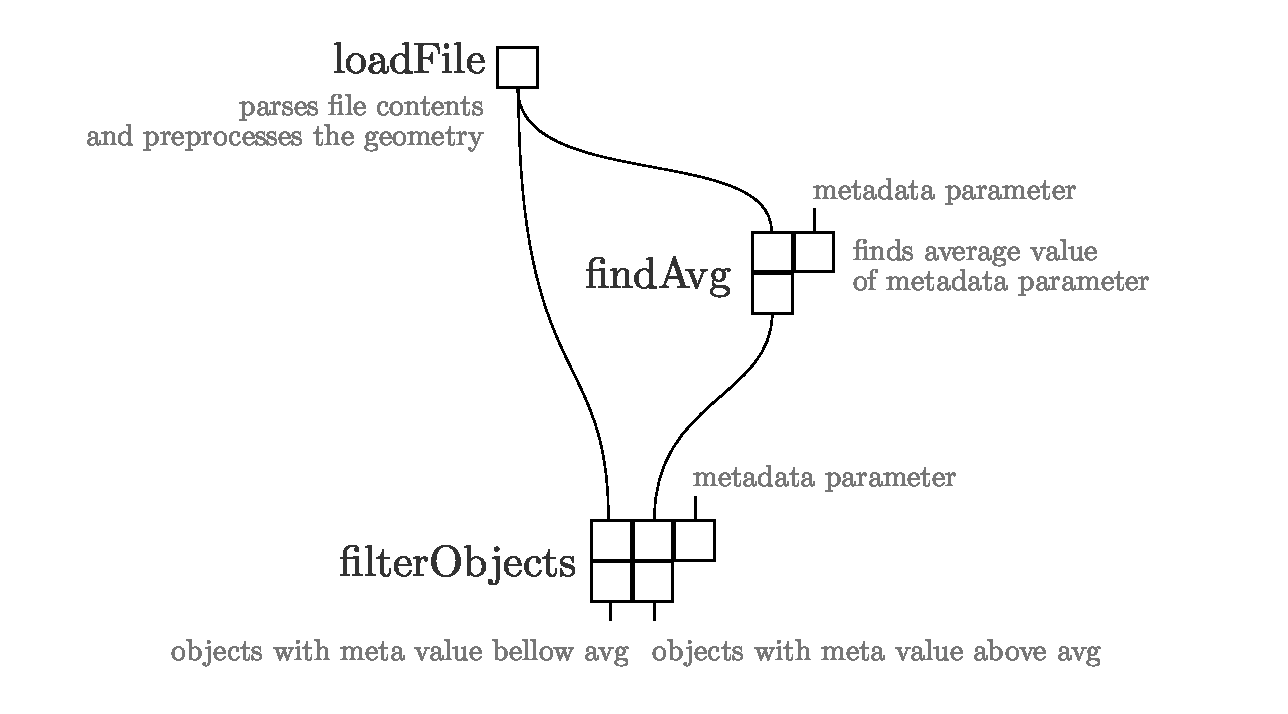
\includegraphics[width=\linewidth]{figures/editor.pdf}
    \caption{Illustration of the proposed editor design}
    \label{fig:editor}
\end{figure}

The assembled pipeline is represented as an acyclic directed graph of functions. Each function is identified by its unique title, and the structure of the function consists of input and output specifications. Each function can have a variable number of inputs and outputs; however, the connectors also need to have a unique name. From the perspective of the editor, it is not important what the function \textit{actually} does. Each of the input and output function connectors also contains meta-information about the supported type. Therefore, the editor is capable of checking the type compliance.    

Additionally, each function is a system \textit{plugin}. The raw editor is implemented as an application with zero user-accessible functionality. However, the system offers a simple API for adding custom functionalities. This design enables the employment of agile development strategies. 

\section{Data Processing}
The data processing component manages the implementation of the available functions and processes the input data. 

\paragraph{Implementing Functions} As presented in the previous section, each function is a custom system plugin implemented as a separate script. The processing component can dynamically update the function implementation based on the user's changes in the source script. This mechanism is not simple to implement; however, the benefits of this approach allow for rapid prototyping of the system. It is desired to integrate development shortcuts (e.g., IDE launch buttons, default function templates) directly into the editor.  

\paragraph{Processing Input Data} When the editor component submits the pipeline graph to the data processing component, the following sequence of steps follows:
\begin{enumerate}
    \item the graph is checked whether it contains any loops
    \item top sort algorithm is performed to generate the order of the function calls
    \item launches the functions in the generated order while keeping track of the input and output parameters  
\end{enumerate} 

As mentioned in \ref{sec:inputrepres}, data loading requires the use of existing file readers. To avoid reimplementing the reader functionality, the technology used to implement the processing component should be compatible with either Python or Java. Further, the non-trivial functionality of dynamic script loading has to be supported in the chosen language. Python has been chosen for the following reasons:
\begin{itemize}[noitemsep]
    \item CityJSON, based on JSON, is easier to parse than XML; the CityJSON reader is implemented in Python
    \item Python supports dynamic module importing by default using the standard \verb|importlib| package
    \item for improved performance, Python can be easily compiled and integrated with C++ code using the \verb|Cython| compiler
\end{itemize}


\section{Web and Projection Views}
Based on the requirements presented in the section \ref{sec:goals}, the view has to be implemented as a web-based application. The section \ref{sec:virtualtools} introduces a wide range of web-based tools for urban data visualization. However, none of these tools is fully suitable for the current use case; from the developer perspective, the most fitting seems to be the Vis.gl Frameworks --- Deck.gl and Luma.gl. Luma.gl provides a wrapper around WebGL API, and Deck.gl implements a layer-based framework for geospatial data visualization. Like every framework, Deck.gl also has limitations: 
\begin{itemize}[noitemsep]
    \item the framework does not provide a way to create a user interface,
    \item when writing custom shaders, not all WebGL features are fully supported and officially documented (e.g., use of textures for displacement),
    \item the developer has no control over the progressive loading of map tiles.
\end{itemize}
It is possible to develop a reasonable prototype using the Deck.gl framework; however, to further optimize the user experience and provide a higher degree of visual customizability, it is suitable to use a general-purpose graphics library, such as WebGL, directly.

The implementation of the projection view is straightforward --- it requires rendering the visualization using orthographical projection. The projection can be further adjusted to comply with the setting of the projector and the physical model. 





